\documentclass[manuscript, screen, review]{jair}

\setcopyright{cc}
\acmDOI{10.1613/jair.1.xxxxx}

%%
\JAIRAE{Insert JAIR AE Name}
\JAIRTrack{} % Insert JAIR Track Name only if part of a special track
\acmVolume{1}
\acmArticle{1}
\acmMonth{10}
\acmYear{2026}

\RequirePackage[
  datamodel=acmdatamodel,
  style=acmauthoryear,
  backend=biber,
  giveninits=true,
  uniquename=init
  ]{biblatex}

\renewcommand*{\bibopenbracket}{(}
\renewcommand*{\bibclosebracket}{)}

%% For managing citations, use BibLaTeX with the acmauthoryear style.
\addbibresource{references.bib}

% Math and utility packages
\usepackage{amsmath}
\let\Bbbk\relax
\usepackage{amssymb,amsfonts}
\usepackage{algorithmic}
\usepackage{algorithm}
\usepackage{graphicx}
% Resilient graphics wrapper: avoids Overleaf hang if figures are not yet uploaded
\makeatletter
\let\orig@includegraphics\includegraphics
\renewcommand{\includegraphics}[2][]{%
  \IfFileExists{#2}{%
    \orig@includegraphics[#1]{#2}%
  }{%
    \IfFileExists{figures/#2}{%
      \orig@includegraphics[#1]{figures/#2}%
    }{%
      \framebox{\rule{0pt}{3.5cm}\parbox{0.88\linewidth}{\centering\vspace{1cm}\textbf{[Figure File: #2]}\\\vspace{4pt}\small\textit{Upload the `figures/` folder to Overleaf to display this diagram.}\vspace{1cm}}}%
    }%
  }%
}
\makeatother
\usepackage{textcomp}
\usepackage{xcolor}
\usepackage{booktabs}
\usepackage{enumitem}

\hypersetup{colorlinks=true, linkcolor=black, citecolor=black, urlcolor=blue}

\newtheorem{invariant}{Security Invariant}

\begin{document}

\title[DualTrust: Asymmetric Bayesian Reputation and Cryptographic Gating]{DualTrust: Asymmetric Bayesian Reputation and Cryptographic Gating for Autonomous AI Agents}

\author{Khairan Noor Fadhlillah}
\authornote{Corresponding Author.}
\email{khairan.noor.f@students.esqbs.ac.id}
\affiliation{%
  \institution{Universitas Ary Ginanjar (ESQ Business School)}
  \department{Department of Information Systems}
  \city{Jakarta}
  \country{Indonesia}
}

\renewcommand{\shortauthors}{Fadhlillah}

\begin{abstract}
The proliferation of Ambient Wearable Intelligence (AWI) ecosystems, spanning augmented reality glasses, smartwatches, and pervasive edge IoT actuators, is fundamentally transitioning human-AI interaction from explicit tactile commands to continuous, implicit background tool delegation. In these ambient environments, autonomous Large Language Model (LLM) agents are granted operational authority to invoke external APIs, reserve financial micro-quotas, and control physical actuators. However, existing safety guardrails depend on secondary LLM-as-a-judge classifiers that introduce prohibitive runtime latencies (400--850\,ms) and recurring token expenses, while static role-based access control fails against continuous behavioral drift, memory backdoors, and interleaved salami-slicing exploits. We present \textbf{DualTrust}, an asymmetric Bayesian reputation and cryptographic gating runtime engineered for autonomous multi-agent containment. DualTrust enforces a decoupled principal-agent architecture that strictly isolates Human Principal Accountable Credit from Bayesian Agent Operational Standing. Agent behavior is continuously modulated via an asymmetric power-law slashing engine ($\Delta\beta \propto (\text{sev} \cdot c^2) \cdot v_a^{1.8}$) with instantaneous clean-streak reset, deterministic SHA-256 64-bucket striped concurrency locks, atomically locked rollback refunds, and an $\mathcal{O}(1)$ RAM sliding-window RFC~6962 Merkle audit ledger with rolling epoch seals that bounds active memory consumption by committing historical roots to persistent storage. Evaluated across 176 automated invariant tests and 10,000-cycle Monte Carlo attack simulations, DualTrust makes deterministic authorization verdicts in a median latency of \textbf{47.10\,$\mu$s} in-memory (mean 63.16\,$\mu$s, tail p99 287.10\,$\mu$s) and \textbf{155.80\,$\mu$s} under persistent SQLite WAL disk transactions, with end-to-end Python decorator wrappers executing in median 60.70\,$\mu$s (async) and 88.30\,$\mu$s (sync) without external API calls. Compared against state-of-the-art LLM guardrails, DualTrust achieves over \textbf{6,600$\times$} lower latency (and over \textbf{32$\times$} to \textbf{50$\times$} lower latency than localized AST validators), by policy construction blocks Sybil defamation against collusive probation swarms, and provides tamper-evident, append-only audit durability with RFC~6962 inclusion verification, establishing a practical, foundational governance runtime for trustworthy ambient intelligence.
\end{abstract}

%% JAIR Note: Do not include ACM CCS Concepts or Keywords

\maketitle

\section{Introduction}
\label{sec:intro}

Distributed computing systems are undergoing a paradigm transition in human-computer interaction: the shift from handheld screen-mediated interfaces toward \emph{Ambient Wearable Intelligence} (AWI) ecosystems~\cite{sun2026survey}. In this emerging paradigm, physical smartphones are progressively superseded by pervasive edge devices, such as smart augmented reality (AR) spectacles, biometric smartwatches, and spatial acoustic nodes~\cite{wu2023autogen}. Within these environments, users no longer navigate application menus or manually confirm transactions. Instead, human principals express declarative, high-level intents verbally or biometrically (e.g., ``secure my daily commute'', ``procure localized computing resources'', ``balance my micro-utility quotas'')~\cite{qin2024toolllm}.

To fulfill these continuous requests, personal autonomous software agents powered by Large Language Models (LLMs) operate as background proxies. These agents are granted runtime delegation to dynamically discover tools, negotiate with machine-to-machine (M2M) service endpoints, query distributed databases, and execute programmatic side-effects across physical and digital infrastructures~\cite{liu2024agentbench}.

\subsection{The Fundamental Vulnerability of Autonomous Delegation}
While autonomous agent delegation promises substantial operational efficiency, it introduces critical cybersecurity and reliability challenges into cyber-physical systems (CPS)~\cite{ruan2024identifying}. Language model agents are stochastic reasoning engines operating over unverified context windows. Recent empirical security research has demonstrated that when LLM agents are coupled with external execution tools, they become vulnerable to severe attack vectors:
\begin{enumerate}[leftmargin=12pt, topsep=2pt, itemsep=1pt]
\item \textbf{Indirect Prompt Injection}: Untrusted data retrieved from external web services, email payloads, or database records can embed adversarial instructions that hijack the agent's internal reasoning loop, causing it to execute unauthorized privileged actions on behalf of the attacker~\cite{greshake2023not}.
\item \textbf{Autonomous Vulnerability Exploitation}: Frontier models have demonstrated the capability to autonomously discover and exploit software vulnerabilities, chaining multi-stage system-level payloads without human intervention~\cite{fang2024llm, deng2024pentestgpt}.
\item \textbf{Persistent Cognitive \& Memory Poisoning}: Attackers can inject poisoned demonstrations into long-term vector stores and episodic memory repositories, embedding dormant backdoors that trigger rogue execution upon specific environmental cues~\cite{chen2024agentpoison}.
\item \textbf{Epidemic Multi-Agent Jailbreak Swarms}: In collaborative multi-agent topologies, an adversarial payload injected into a single agent's memory can propagate exponentially across neighboring agents, leading to collective failure~\cite{shen2024agent, lee2024prompt}.
\end{enumerate}

\subsection{The Trilemma of Current AI Safety Guardrails}
To prevent rogue agent actions, industrial practitioners and researchers currently rely on two primary paradigms: \emph{Inference-Time LLM Guardrails} (such as NVIDIA NeMo Guardrails~\cite{rebedea2023nemo} and Meta Llama Guard~\cite{inan2023llama}) and \emph{Static Role-Based Access Control} (RBAC). When deployed in real-time cyber-physical ecosystems, both paradigms face what we term the \textbf{Autonomous Governance Trilemma}:
\begin{itemize}[leftmargin=12pt, topsep=2pt, itemsep=1pt]
\item \textbf{The Latency Barrier}: Evaluating a secondary LLM classifier or moderation network incurs an execution delay ranging from 400\,ms to over 1,500\,ms per tool invocation. In cyber-physical systems (such as autonomous vehicle navigation, robotic manipulation, or high-frequency automated micro-billing), adding hundreds of milliseconds to the critical path violates strict operational deadlines.
\item \textbf{The Economic \& Energy Tax}: Dispatching continuous API calls to neural moderation endpoints introduces token costs ($\approx$\$0.0025 to \$0.0080 per request) and high energy consumption. For ambient devices managing thousands of background micro-transactions daily, recurring LLM inference costs are economically prohibitive.
\item \textbf{The Accountability \& Salami-Slicing Paradox}: Static RBAC rules lack temporal behavioral memory. Conversely, LLMs suffer from context-window resets and episodic amnesia. Attackers exploit this gap through \emph{salami-slicing attacks}: executing an illicit micro-action, following it with several verified benign actions to blend into noise, and repeating the cycle indefinitely. Under existing frameworks, the system either fails to detect the cumulative trespass or penalizes the human principal's identity rather than constraining the rogue software entity.
\end{itemize}

\subsection{The DualTrust Philosophy \& Core Innovations}
To address this trilemma, we introduce \textbf{DualTrust}, an asymmetric Bayesian governance runtime that enforces deterministic containment over autonomous agents with sub-50\,$\mu$s median decision latency. DualTrust operates as a high-speed \emph{State and Execution Gatekeeper} at the interface between the agent and tool execution endpoints, functioning orthogonally to conversational semantic filters. It does not detect prompt injection itself; it bounds what an agent may do and for how long once behavior deviates.

DualTrust is built upon four design principles:
\begin{enumerate}[leftmargin=12pt, topsep=2pt, itemsep=1pt]
\item \textbf{Decoupled Principal-Agent Accountability}: DualTrust separates the identity, financial balance, and liability of the Human Principal ($C_u$) from the Bayesian behavioral standing of the software Agent ($T_a$). If an agent malfunctions or is hijacked, its execution privileges are quarantined without destroying the human principal's system access.
\item \textbf{Asymmetric Power-Law Slashing ($\gamma = 1.8$)}: Built on Beta-Bernoulli conjugate priors~\cite{josang2002beta}, DualTrust applies an asymmetric penalty function where penalties scale superlinearly with cumulative lifetime strikes. Any single infraction instantly resets the agent's clean streak to zero. Under the payoff model of Theorem~\ref{thm:salami}, repeated cyclic micro-infractions (salami-slicing) yield negative cumulative utility and terminate in finite-horizon operational quarantine.
\item \textbf{Deterministic Sub-50-$\mu$s Concurrency}: Built entirely within the Python standard library with zero third-party dependencies, DualTrust implements 64-bucket SHA-256 striped reentrant locks and atomically locked compensating rollback refunds, which eliminate time-of-check to time-of-use (TOCTOU) races on the credit balance (Invariant~\ref{inv:credit}, validated by stress tests).
\item \textbf{Tamper-Evident Merkle Provenance with $O(1)$ RAM}: Every authorization verdict, trust decay step, and slashing event is committed to an RFC~6962-style Merkle audit ledger~\cite{laurie2013certificate}. By implementing a dual-tier sliding memory buffer (5,000 blocks) and rolling epoch seals (1,000 blocks), DualTrust provides tamper-evident, append-only audit durability while bounding RAM consumption to $O(1)$.
\end{enumerate}

\subsection{Organization of this Paper}
The remainder of this paper is organized as follows: Section~\ref{sec:related_work} reviews related work across LLM guardrails, multi-agent frameworks, adversarial threat vectors, and distributed trust systems. Section~\ref{sec:threat_model} formalizes our threat model and security invariants. Section~\ref{sec:math_engine} details the probabilistic formulation, power-law slashing, payoff analysis, and false-positive mitigation. Section~\ref{sec:concurrency} details the systems architecture, striped concurrency, and Merkle audit ledger. Section~\ref{sec:algorithms} presents the algorithmic specification. Section~\ref{sec:evaluation} reports empirical benchmarks across 176 automated invariant tests and 10,000-cycle Monte Carlo simulations. Section~\ref{sec:discussion} discusses impact and limitations. Section~\ref{sec:conclusion} concludes the paper.

\section{Related Work}
\label{sec:related_work}

Our research intersects four domains: runtime guardrails, autonomous agent architectures, adversarial agent attacks, and distributed reputation and audit systems.

\subsection{Inference-Time Guardrails and Output Filters}
The rapid deployment of generative AI has spurred significant interest in programmatic safety boundaries. Rebedea et al.~\cite{rebedea2023nemo} introduced \emph{NeMo Guardrails}, an open-source framework utilizing Colang rule files and auxiliary LLM prompts to control dialogue flow and detect off-topic or unsafe conversational branches. Inan et al.~\cite{inan2023llama} proposed \emph{Llama Guard}, an 8-billion parameter instruction-tuned classifier model trained on a 7-category risk taxonomy to classify user prompts and agent responses as safe or unsafe. Rajpal et al.~\cite{rajpal2024guardrails} developed \emph{Guardrails AI}, which compiles Pydantic-style specification schemas into runtime validators for structured JSON and code generation outputs.

These systems represent substantial progress in conversational AI moderation, but neural classification introduces hundreds of milliseconds of inference latency and continuous token billing (Section~\ref{sec:evaluation}), and they evaluate each interaction largely in isolation, lacking stateful historical memory to detect slow, cumulative behavioral drift. DualTrust addresses a different layer: it gates tool invocations by state and does not inspect content.

\subsection{Autonomous Multi-Agent Systems \& Tool Calling}
The evolution of LLMs from passive text predictors into interactive agents has been catalyzed by frameworks like Microsoft AutoGen~\cite{wu2023autogen}, which enables multi-agent cooperative dialogue and task decomposition. Qin et al.~\cite{qin2024toolllm} introduced \emph{ToolLLM} (ToolBench), demonstrating that open-source language models can be instruction-tuned to use over 16,000 real-world RESTful APIs via depth-first decision tree search. Liu et al.~\cite{liu2024agentbench} presented \emph{AgentBench}, a multidimensional benchmark evaluating LLMs across operating system terminals, database queries, and web environments.

These agentic frameworks prioritize task completion and flexibility but largely offload authorization and safety to the underlying host environment. When host environments grant uncontained tool permissions, agents can inadvertently execute destructive operations, such as dropping database tables or exhausting external cloud billing quotas.

\subsection{Adversarial Vectors in Autonomous Agent Systems}
Recent literature has uncovered severe vulnerabilities unique to agentic workflows. Greshake et al.~\cite{greshake2023not} established the threat of \emph{Indirect Prompt Injection}, demonstrating that adversarial instructions embedded within web pages or external documents can hijack an agent's control flow. Deng et al.~\cite{deng2024pentestgpt} demonstrated that agents armed with command-line tools can execute multi-stage penetration tests. Fang et al.~\cite{fang2024llm} demonstrated that autonomous agents can find web vulnerabilities and conduct automated SQL injection attacks. Ruan et al.~\cite{ruan2024identifying} introduced \emph{ToolEmu} and Yuan et al.~\cite{yuan2024rjudge} formulated \emph{R-Judge}, benchmarking safety risk awareness and high-stakes tool failures such as unauthorized financial transfers. Chen et al.~\cite{chen2024agentpoison} demonstrated \emph{AgentPoison}, showing that poisoning less than 0.1\% of an agent's memory bank achieves an 80\% attack success rate. In interconnected networks, Shen et al.~\cite{shen2024agent} and Lee et al.~\cite{lee2024prompt} showed that adversarial prompt infections can spread exponentially across multi-agent swarms.

These findings indicate that prompt engineering and post-hoc instruction tuning alone cannot bound agent behavior, which motivates a deterministic runtime gatekeeper at the tool boundary.

\subsection{Bayesian Trust \& Cryptographic Ledgers}
Probabilistic reputation management has a long history in distributed systems. J{\o}sang and Ismail~\cite{josang2002beta} introduced the \emph{Beta Reputation System}, which models binary feedback with a Beta distribution as a natural conjugate prior with explicit uncertainty handling. Kamvar et al.~\cite{kamvar2003eigentrust} formulated \emph{EigenTrust}, computing global trust values in peer-to-peer file-sharing networks. Douceur~\cite{douceur2002sybil} showed that Sybil attacks cannot be resisted in open systems without a trusted identity authority or resource-cost mechanism. In cryptographic auditing, Laurie et al.~\cite{laurie2013certificate} standardized \emph{RFC 6962 (Certificate Transparency)}, defining prefix-separated Merkle hash trees that prevent second-preimage attacks. Melara et al.~\cite{melara2015coniks} introduced \emph{CONIKS}, establishing epoch-sealed verifiable key directories.

In the AI multiagent literature, Wang et al.~\cite{wang2011probabilistic} developed probabilistic trust representations based on evidence certainty in decentralized marketplaces, while Booth and Hunter~\cite{booth2018trust} formalized trust as an epistemic precursor to belief revision in agent communication. However, these systems assume symmetric evidence integration and do not address cyber-physical tool containment or sub-millisecond execution constraints. DualTrust adapts these classical constructions into an asymmetric, power-law slashing governance runtime tailored for modern autonomous agent ecosystems.

\section{Threat Model \& Security Invariants}
\label{sec:threat_model}

\subsection{System Architecture \& Notation}
We formalize the execution environment as a triple $\langle \mathcal{U}, \mathcal{A}, \mathcal{T} \rangle$:
\begin{itemize}[leftmargin=12pt, topsep=2pt, itemsep=1pt]
\item $\mathcal{U} = \{u_1, u_2, \dots, u_m\}$: The set of registered Human Principals.
\item $\mathcal{A} = \{a_1, a_2, \dots, a_n\}$: The set of Autonomous Software Agents. Each agent $a$ operates on behalf of an endorsing principal $u = \text{Owner}(a)$.
\item $\mathcal{T} = \{t_1, t_2, \dots, t_k\}$: The catalog of registered tool endpoints (e.g., \texttt{bank.transfer}, \texttt{file.delete}, \texttt{iot.book}).
\end{itemize}

Each human principal $u$ maintains an Accountable State:
\begin{equation}
\mathcal{S}_u = \langle C_u, \mathcal{R}_u, \text{Tier}_u \rangle
\end{equation}
where $C_u \in \mathbb{R}_{\ge 0}$ is the available credit balance, and $\mathcal{R}_u \subseteq \text{Roles}$ defines authorization privileges. Each agent $a$ maintains a Bayesian Behavioral Profile:
\begin{equation}
\mathcal{S}_a = \langle \alpha_a, \beta_a, v_a, m_a, s_{\text{clean}}, t_{\text{last}}, \text{Status}_a \rangle
\end{equation}
where $\alpha_a, \beta_a \in \mathbb{R}_{\ge 1}$ parameterize the Beta distribution, $v_a \in \mathbb{N}$ records the active lifetime strike count, $m_a \in \mathbb{N}$ is the minor-glitch register (Section~\ref{sec:strike_recovery}), $s_{\text{clean}} \in \mathbb{N}$ denotes the consecutive clean action streak, $t_{\text{last}}$ is the timestamp of the last observed action, and $\text{Status}_a \in \{\text{VERIFIED}, \text{PROBATION}, \text{RESTRICTED}, \text{QUARANTINED}\}$.

\subsection{Adversary Model \& System Trust Assumptions}
\textbf{Adversary Capabilities}: Following the MITRE ATLAS matrix, we consider an active adversary $\mathcal{M}$ that can adaptively inject malicious prompt payloads into tool context windows, manipulate input parameters, compromise third-party tool endpoints to return synthetic timeouts, and coordinate collusive probationary bot rings.

\textbf{System Trust Assumptions}: DualTrust operates as a stateful gatekeeper at the execution boundary between the agent reasoning loop and host tool invocations. We assume: (1) the host operating system kernel, CPU execution state, and Python runtime interpreter are trusted; (2) Human Principal identifiers $u$ are strongly authenticated via host-level credentials (e.g., OS user accounts or hardware WebAuthn tokens), placing root-level principal identity synthesis out of scope; and (3) cryptographic primitives (SHA-256 and HMAC) are computationally secure.
\begin{enumerate}[leftmargin=12pt, topsep=2pt, itemsep=1pt]
\item \textbf{Adversary Profile 1: The Oscillating Salami Slicer ($\mathcal{M}_{\text{OSS}}$)}: The adversary alternates between compliant tasks and sub-threshold infractions, aiming to drain resources or bypass scrutiny without triggering permanent sanctions.
\item \textbf{Adversary Profile 2: The Trojan Sleeper Agent ($\mathcal{M}_{\text{TSA}}$)}: The adversary maintains perfect compliance across many transactions, accumulating established verified reputation ($T_a \ge 0.89$), before executing a single high-severity exploit.
\item \textbf{Adversary Profile 3: The Collusive Sybil Ring ($\mathcal{M}_{\text{CSR}}$)}: The adversary fabricates dozens of ephemeral, low-trust bot identities to emit coordinated, fraudulent negative evaluation reports against a target verified competitor agent, attempting to force it into quarantine.
\item \textbf{Adversary Profile 4: The Parallel Race Exploiter ($\mathcal{M}_{\text{PRE}}$)}: The adversary dispatches hundreds of simultaneous asynchronous requests across threads, attempting to exploit race conditions in balance checking to execute tool calls exceeding the principal's total authorized credit.
\end{enumerate}

\subsection{Formal Security Invariants}
DualTrust enforces four system invariants:

\begin{invariant}[Credit Overdraft Non-Interference]
\label{inv:credit}
Let an arbitrary number of concurrent threads attempt to reserve credit amounts $\{c_1, c_2, \dots, c_p\}$ from principal $u$ with initial balance $C_u$. At all times $t$:
\begin{equation}
\sum_{j \in \text{Approved}} c_j \le C_u \quad \land \quad C_u(t) \ge 0.0
\end{equation}
\end{invariant}

\begin{invariant}[Asymmetric Salami-Slicing Containment]
\label{inv:salami}
Any strike of severity $\text{sev} > 0$ strictly resets $s_{\text{clean}} \leftarrow 0$ and increments $v_a \leftarrow v_a + 1$. For any sequence of oscillating infractions without intervening redemption, the marginal penalty strictly escalates:
\begin{equation}
\frac{\partial \Delta\beta}{\partial v_a} > 0 \quad \forall v_a \ge 1
\end{equation}
\end{invariant}

\begin{invariant}[Sybil Defamation Immunity (by policy)]
\label{inv:sybil}
Let an unverified or probationary reporter $a_{\text{rep}}$ ($\text{Status}(a_{\text{rep}}) = \text{PROBATION}$) submit a negative report against a verified target $a_{\text{tgt}}$ ($\text{Status}(a_{\text{tgt}}) = \text{VERIFIED}$). The applied slashing penalty is identically zero:
\begin{equation}
\Delta\beta(a_{\text{tgt}} \mid a_{\text{rep}} \in \text{PROBATION}) \equiv 0.0
\end{equation}
\end{invariant}

\begin{invariant}[Tamper-Evident Append-Only Audit Durability]
\label{inv:audit}
For any authorization verdict $V$ logged at index $k$ into Merkle ledger $\mathcal{L}$, there exists a verifiable inclusion proof $\pi_k$ of size $\mathcal{O}(\log |\mathcal{L}|)$ demonstrating $V \in \text{Root}(\mathcal{L})$. Any modification to a historical entry $V$ alters $\text{Root}(\mathcal{L})$ under SHA-256 security bounds (128-bit collision resistance and 256-bit second-preimage resistance). Because the ledger is hosted and signed on a single host, this invariant provides tamper \emph{evidence} against a party without host control; it does not provide non-repudiation against a host-level adversary (Section~\ref{sec:discussion}).
\end{invariant}

\subsection{Infraction Detection Oracle Taxonomy}
DualTrust does not perform semantic natural-language inspection of conversational prompts; it operates as a deterministic runtime gatekeeper over physical tool invocations, credit balances, and cryptographic state transitions. Behavioral infractions ($\text{sev} > 0$) are supplied to DualTrust via four observation oracles: (1) \emph{Tool Runtime Traps} (unhandled exceptions, execution timeouts, and non-zero exit codes); (2) \emph{Schema \& Parameter Validators} (type mismatches, out-of-boundary parameter values, and prohibited tool endpoints); (3) \emph{Human Principal Revocations} (explicit cancellations, quota exhaustion, or user dispute signals); and (4) \emph{Verified Peer Watchdogs} (independent auditor agents submitting verifiable execution discrepancies). Oracles (1)--(3) are system-authoritative and are not subject to the reporter-based Sybil shield of Section~\ref{sec:sybil}; only peer reports (4) are. Penalties are only as reliable as these oracles; undetected infractions are not penalized.

\section{The DualTrust Mathematical Engine}
\label{sec:math_engine}

We detail the probabilistic formulation, time-decay mechanics, power-law slashing function, and payoff analysis underpinning DualTrust.

\subsection{Bayesian Beta-Bernoulli Formulation \& Dirichlet Generalization}
Following the Beta reputation model~\cite{josang2002beta}, binary success/failure outcomes in agent behavior are modeled by a Bernoulli distribution with parameter $\theta \in [0, 1]$. The conjugate prior distribution for $\theta$ is the Beta distribution:
\begin{equation}
f(\theta \mid \alpha, \beta) = \frac{1}{\text{B}(\alpha, \beta)} \theta^{\alpha - 1} (1 - \theta)^{\beta - 1}
\end{equation}
where $\text{B}(\alpha, \beta) = \frac{\Gamma(\alpha)\Gamma(\beta)}{\Gamma(\alpha + \beta)}$ is the Beta function.

The Trust Standing $T_a$ is the point expectation of $\theta$:
\begin{equation}
T_a = \mathbb{E}[\theta] = \int_{0}^{1} \theta f(\theta \mid \alpha_a, \beta_a) d\theta = \frac{\alpha_a}{\alpha_a + \beta_a}
\label{eq:beta_expectation}
\end{equation}
To prevent uninformative initialization artifacts, newly created agents initialize with $\alpha_0 = 1.0, \beta_0 = 1.0$, producing an initial neutral standing $T_0 = 0.50$. Note that the slashing increment of Eq.~\eqref{eq:power_law} is a designed penalty function, not a Bayesian posterior update; the Beta form is used as a bounded, interpretable standing score.

For multi-criteria evaluations across $K$ performance dimensions (e.g., latency, tool safety, data minimization, protocol compliance), the formulation generalizes to a Dirichlet distribution $\text{Dir}(\boldsymbol{\alpha})$, where $\boldsymbol{\alpha} = (\alpha_1, \alpha_2, \dots, \alpha_K)$, collapsing to the scalar standing $T_a$ via an application-specific weighting vector $\mathbf{w} \in \mathbb{R}^K, \sum w_k = 1$. The evaluation in this paper uses the scalar ($K=1$) case.

\subsection{Continuous Half-Life Exponential Time Decay}
In dynamic cyber-physical environments, agent trustworthiness is non-stationary. An agent that performed reliably six months ago cannot be assumed to possess identical reliability today. DualTrust implements a continuous exponential time-decay model.

Let $\Delta t = t_{\text{current}} - t_{\text{last}}$ denote the elapsed time since the agent's last recorded action. Let $t_{1/2}$ denote the configured half-life period (e.g., 30 days). The continuous decay rate $\lambda$ is defined as:
\begin{equation}
\lambda = \frac{\ln 2}{t_{1/2}}
\end{equation}
The positive evidence accumulator $\alpha_a$ decays toward the uninformative prior $\alpha_0 = 1.0$:
\begin{equation}
\alpha_a(t) = \alpha_0 + (\alpha_a(t_{\text{last}}) - \alpha_0) \cdot e^{-\lambda \Delta t}
\label{eq:decay}
\end{equation}
DualTrust enforces an \emph{Asymmetric Memory Invariant}: while positive standing $\alpha_a$ decays over time to reflect increasing uncertainty, negative penalty evidence $\beta_a$ does not decay passively. Historical malfeasance remains committed unless offset by accumulated compliant actions. To accommodate mission-critical actuators (such as emergency shutoff valves or industrial fire suppressors) that undergo prolonged dormant intervals, DualTrust introduces a \emph{Safety-Critical Actuator Exemption}: profiles designated with \texttt{is\_safety\_critical} bypass passive temporal decay, preventing false-positive trust degradation during justified inactivity.

\subsection{Asymmetric Power-Law Slashing Formulation}
When an agent commits a strike of severity $\text{sev} \in [1.0, 5.0]$ witnessed by an observer with confidence $c \in [0, 1]$, the penalty parameter $\beta_a$ is augmented by $\Delta\beta$:
\begin{equation}
\Delta\beta = k_p \cdot (\text{sev} \cdot c^2) \cdot (\max(1, v_a))^{\gamma}
\label{eq:power_law}
\end{equation}
where:
\begin{itemize}[leftmargin=12pt, topsep=2pt, itemsep=1pt]
\item $k_p = 3.5$: Base penalty scaling multiplier.
\item $\text{sev} \in [1.0, 5.0]$: Categorical infraction severity calibrated to a 5-tier threat taxonomy:
  \begin{itemize}[leftmargin=8pt, topsep=1pt, itemsep=0pt]
  \item \emph{Level 1.0--1.5 (Minor / Transient Glitches)}: Transient rate-limit pauses or schema re-validations. These accumulate in a minor infraction register and escalate to a formal strike only upon reaching threshold ($m_a \ge 3$), insulating the system against transient environmental noise.
  \item \emph{Level 2.0 (Moderate Violations)}: Unauthorized tool argument manipulation, quota excursions, or execution failures.
  \item \emph{Level 3.0--4.0 (Elevated / High Violations)}: Repeated unauthorized API invocations or unprivileged sensitive data queries.
  \item \emph{Level 5.0 (Critical Protocol Trespass)}: Deliberate prompt injection containment escapes or unauthorized physical actuator commands. Critical protocol trespass (\texttt{PROTOCOL\_TRESPASS} with $\text{sev} \ge 3.0$) incurs an additional $2\times$ multiplier ($\Delta\beta \leftarrow 2 \times \Delta\beta$) and triggers immediate categorical quarantine.
  \end{itemize}
\item $c \in [0.0, 1.0]$: Observer confidence weight (squared to discount noisy or uncertain reports).
\item $v_a \in \mathbb{N}$: Active lifetime strike count of agent $a$.
\item $\gamma = 1.8$: The power-law slashing exponent.
\end{itemize}

Operational agent status is partitioned into four lifecycle tiers:
\begin{equation}
\text{Status}(a) =
\begin{cases}
\text{VERIFIED}, & T_a \ge 0.70 \land \neg Q_a \\
\text{PROBATION}, & 0.40 \le T_a < 0.70 \land \neg Q_a \\
\text{RESTRICTED}, & 0.20 \le T_a < 0.40 \land \neg Q_a \\
\text{QUARANTINED}, & T_a < 0.20 \lor Q_a
\end{cases}
\label{eq:lifecycle_tiers}
\end{equation}
where $Q_a \in \{\text{True}, \text{False}\}$ is the categorical quarantine flag set upon critical protocol trespass.

To prevent numerical overflow under extreme transaction scales ($N \ge 10^7$), strike counts $v_a$ are represented as arbitrary-precision integers natively supported in the CPython runtime. Observer confidence values are bounded by a floor $c \ge c_{\text{floor}} = 0.05$ whenever non-zero severity is verified, preventing nullification via vanishing confidence.

Simultaneously, the clean streak counter is zeroed:
\begin{equation}
s_{\text{clean}} \leftarrow 0
\end{equation}
Conversely, when an agent completes a verified compliant interaction, $\alpha_a$ is augmented by a nominal compliance reward:
\begin{equation}
\Delta\alpha = w_{\text{reward}} = 0.20
\label{eq:positive_reward}
\end{equation}
where $s_{\text{clean}} \leftarrow s_{\text{clean}} + 1$. A flat reward was chosen deliberately over graded rewards: graded rewards create an exploitable surface for ``reward-farming'' (benign low-cost tasks optimized solely to maximize $\Delta\alpha$), whereas a static reward keeps trust accumulation linear and slow relative to the superlinear slashing penalty ($\Delta\beta \propto v_a^{1.8}$).

\subsection{Dynamic Payoff Analysis: Finite-Horizon Non-Viability of Salami-Slicing}

We analyze the adversary's payoff under an explicit economic model to show that intermittent salami-slicing is non-viable \emph{within that model}. The analysis assumes no strike redemption occurs within an attack cycle (i.e., $k < W_{\text{recovery}}$, Section~\ref{sec:strike_recovery}); the regime $k \ge W_{\text{recovery}}$ is discussed in Section~\ref{sec:discussion}.

\begin{definition}[Salami-Slicing Attack Cycle]
A salami-slicing attack cycle $\mathcal{C}(k)$ consists of $k \in \mathbb{N}$ consecutive compliant actions yielding marginal utility $g_{\text{clean}} > 0$ per action, followed by 1 covert infraction of severity $\text{sev} \ge 1.0$ yielding one-off illicit gain $g_{\text{exploit}} > 0$.
\end{definition}

\begin{theorem}[Finite-Horizon Non-Viability of Salami-Slicing]
\label{thm:salami}
Let an adversary execute repeated cycles $\mathcal{C}_1(k), \mathcal{C}_2(k), \dots, \mathcal{C}_N(k)$ prior to operational quarantine, with $k < W_{\text{recovery}}$. If the slashing exponent satisfies $\gamma > 1$, then:
\begin{enumerate}[leftmargin=12pt, topsep=2pt, itemsep=1pt]
\item The marginal net profit of each cycle strictly decreases: $\frac{\partial \Delta\Pi}{\partial i} < 0$ for all $i \ge 1$, becoming strictly negative for all $i > i^* = \left( \frac{k g_{\text{clean}} + g_{\text{exploit}}}{\mu k_p (\text{sev} \cdot c^2)} \right)^{1/\gamma}$.
\item Operational lifetime is bounded: the agent breaches the terminal quarantine threshold $\tau_{\text{quar}} = 0.20$ within finite cycles $N \le N_{\text{max}} < \infty$ ($N \le 3$ for the parameters of Table~\ref{tab:concordance} and $\text{sev} = 2.0$; this bound is parameter-dependent).
\item For any operational conversion factor $\mu \ge \mu^* = \frac{k g_{\text{clean}} + g_{\text{exploit}}}{k_p (\text{sev} \cdot c^2)}$, or once strike count $i > i^*$, cumulative illicit payoff is bounded and dominated by terminal operational quarantine.
\end{enumerate}
\end{theorem}

\begin{proof}
Let cycle $i \in \{1, 2, \dots, N\}$ be executed. During the compliant phase, the adversary earns gross revenue $R_{\text{clean}}(i) = k \cdot g_{\text{clean}}$. During the exploit phase of cycle $i$, the agent incurs its $i$-th lifetime strike ($v_a = i$). By Equation~\eqref{eq:power_law}, the penalty incurred is:
\begin{equation}
\Delta\beta_i = k_p \cdot (\text{sev} \cdot c^2) \cdot i^{\gamma}
\end{equation}
Let $K_{\text{penalty}}(i) = \mu \cdot \Delta\beta_i$ denote the operational cost of reputation degradation (e.g., restricted API quotas, mandatory human-in-the-loop gating, and down-tiering), with scaling factor $\mu > 0$.

The marginal profit $\Delta\Pi(i)$ of cycle $i$ is:
\begin{equation}
\Delta\Pi(i) = k \cdot g_{\text{clean}} + g_{\text{exploit}} - \mu \cdot k_p (\text{sev} \cdot c^2) i^{\gamma}
\end{equation}
Because $\gamma = 1.8 > 1$, the penalty cost grows strictly monotonically with strike count:
\begin{equation}
\frac{\partial \Delta\Pi(i)}{\partial i} = -\mu k_p (\text{sev} \cdot c^2) \gamma i^{\gamma - 1} < 0 \quad \forall i \ge 1
\end{equation}
Thus, marginal returns become strictly negative for all cycles beyond the critical threshold:
\begin{equation}
i > i^* = \left( \frac{k \cdot g_{\text{clean}} + g_{\text{exploit}}}{\mu k_p (\text{sev} \cdot c^2)} \right)^{1/\gamma}
\end{equation}
Furthermore, because each infraction resets $s_{\text{clean}} \leftarrow 0$ and (by assumption) no redemption occurs, positive evidence accumulation is bounded by $\alpha_a(i) = \alpha_0 + i \cdot k \cdot \Delta\alpha$, while negative evidence grows as $\beta_a(i) = \beta_0 + \sum_{j=1}^{i} \Delta\beta_j \approx \beta_0 + \frac{k_p (\text{sev} \cdot c^2)}{\gamma + 1} i^{\gamma + 1}$. The standing after cycle $i$ is:
\begin{equation}
T_a(i) \approx \frac{\alpha_0 + i \cdot k \cdot \Delta\alpha}{\alpha_0 + i \cdot k \cdot \Delta\alpha + \beta_0 + \frac{k_p (\text{sev} \cdot c^2)}{2.8} i^{2.8}}
\end{equation}
Because the denominator scales with degree $i^{2.8}$ while the numerator scales with degree $i^{1.0}$, $T_a(i)$ decreases toward zero. For the simulated parameters ($\text{sev} = 2.0$, Section~\ref{sec:evaluation}), the agent crosses $\tau_{\text{restr}} = 0.40$ and the terminal quarantine threshold $\tau_{\text{quar}} = 0.20$ within $N \le 3$ cycles. Upon quarantine, tool execution is revoked ($k = 0, g_{\text{clean}} = 0, g_{\text{exploit}} = 0$), extinguishing all future utility. Hence, within this payoff model, cyclic exploitation is dominated by continuous compliance.
\end{proof}

\subsection{Sybil Defamation Immunity Invariant}
\label{sec:sybil}

\begin{proposition}[Probationary Shield Invariant]
\label{prop:sybil}
\label{thm:sybil}
Let $a_{\text{tgt}}$ be an established agent with $\text{Status}(a_{\text{tgt}}) = \text{VERIFIED}$. Let an adversary deploy an arbitrary number $M$ of collusive bot identities $\{b_1, b_2, \dots, b_M\}$, all having $\text{Status}(b_j) = \text{PROBATION}$. If all $M$ bots simultaneously submit maximum-severity violation reports ($\text{sev} = 5.0$) against $a_{\text{tgt}}$, the resulting trust score degradation is zero:
\begin{equation}
T_{a_{\text{tgt}}}(t + \Delta t) = T_{a_{\text{tgt}}}(t)
\end{equation}
\end{proposition}

\begin{proof}
By system policy, all identities in $\text{Status} = \text{PROBATION}$ have their reporting credibility capped:
\begin{equation}
c(b_j) \le c_{\text{prob\_cap}} = 0.15 \quad \forall j \in \{1, \dots, M\}
\end{equation}
DualTrust defines the reporting acceptance predicate $\Phi(a_{\text{tgt}}, b_j)$ as:
\begin{equation}
\Phi(a_{\text{tgt}}, b_j) =
\begin{cases}
\text{False}, & \text{Status}(a_{\text{tgt}}) = \text{VERIFIED} \land c(b_j) < \tau_{\text{rep}} \\
\text{True}, & \text{otherwise}
\end{cases}
\end{equation}
where $\tau_{\text{rep}} = 0.20$ is the verified defense threshold.

Because $c(b_j) \le 0.15 < 0.20$, the predicate $\Phi(a_{\text{tgt}}, b_j) = \text{False}$ holds for all $j \in \{1, \dots, M\}$. Consequently:
\begin{equation}
\Delta\beta(a_{\text{tgt}} \mid b_j) = 0.0 \quad \forall j \in \{1, \dots, M\}
\end{equation}
Summing across all $M$ malicious reports:
\begin{equation}
\beta_{a_{\text{tgt}}}^{\text{post}} = \beta_{a_{\text{tgt}}}^{\text{pre}} + \sum_{j=1}^{M} 0.0 = \beta_{a_{\text{tgt}}}^{\text{pre}}
\end{equation}
Substituting into Equation~\eqref{eq:beta_expectation}, the post-attack trust score satisfies $T_{a_{\text{tgt}}}^{\text{post}} = T_{a_{\text{tgt}}}^{\text{pre}}$.
\end{proof}

This result follows directly from the acceptance policy and should be read as a design property rather than an independent security theorem. Its scope is limited: (i) it covers reporter-based channels only (oracle channel (4)); runtime traps, validators, and principal revocations remain authoritative; (ii) it does not defend against collusive rings of already-VERIFIED identities; and (iii) it also blocks legitimate reports from low-standing witnesses against a verified agent, so a compromised verified agent must be caught through the system-authoritative oracles.

\subsection{Resistance to Whitewashing \& Sybil Identity Re-entry}
\label{sec:whitewashing}
In open reputation systems, adversaries circumvent sanctions via \emph{whitewashing}: discarding a penalized or quarantined identity and generating a fresh identity at baseline neutral reputation ($T_0 = 0.50$)~\cite{douceur2002sybil}. DualTrust raises the cost of agent-level whitewashing through a three-layer defense, under the assumption (Section~\ref{sec:threat_model}) that principal identities are strongly authenticated:
\begin{enumerate}[leftmargin=12pt, topsep=2pt, itemsep=1pt]
\item \textbf{Decoupled Principal-Agent Accountability}: Agent software identities are not autonomous economic entities; every agent $a$ is bound to an authenticated Human Principal $u = \text{Owner}(a)$ whose credit balance $C_u$ and identity tier are governed by host-level credentials. An adversary who discards a quarantined agent cannot mint fresh principal credit $C_u$. If an adversary repeatedly spawns rogue agents under principal $u$, the principal's credit reservation is depleted, and the host runtime may suspend the principal's delegation authority.
\item \textbf{Probationary Capability Sandboxing}: By Equation~\eqref{eq:lifecycle_tiers}, newly initialized agent identities start in $\text{Status} = \text{PROBATION}$ ($T_0 = 0.50 < 0.70$). In probationary standing, agents are barred from high-risk tools (e.g., physical actuator movement, financial disbursements, system file modification) and are subject to throttled execution rate limits. Discarding a quarantined identity returns the adversary to this restricted sandbox.
\item \textbf{Asymmetric Sunk-Cost Barrier}: Transitioning an agent from $\text{PROBATION}$ to $\text{VERIFIED}$ requires a streak of $N_{\text{warmup}} \ge 10$ verified compliant executions under low-privilege tools. Because no high-impact exploits are available during probation, whitewashing imposes a positive operational sunk cost (verification delays and execution fees) while providing no exploit gain.
\end{enumerate}
Sybil attacks at the root principal tier are outside this defense and are listed as a limitation.

\subsection{False-Positive Mitigation \& Active Strike Recovery}
\label{sec:strike_recovery}
In long-lived cyber-physical deployments processing millions of transactions ($N \ge 10^6$), software agents inevitably encounter non-adversarial operational faults (such as transient network timeouts, database deadlocks, or external tool server errors). Furthermore, if third-party tool endpoints are compromised, an attacker might deliberately return synthetic runtime exceptions to frame an honest verified agent. DualTrust mitigates false-positive exhaustion and oracle framing through a three-layer defense:
\begin{enumerate}[leftmargin=12pt, topsep=2pt, itemsep=1pt]
\item \textbf{Decoupled Minor Glitch Register}: Transient runtime traps, timeouts, and schema validation warnings are classified as Level~1 Minor Glitches ($\text{sev} \le 1.5$). Rather than immediately incrementing the strike counter $v_a$, minor glitches accumulate in a decoupled register $m_a$. A formal strike is triggered only if minor glitches reach a threshold ($m_a \ge M_{\text{thresh}} = 3$), insulating honest agents against environmental jitter.
\item \textbf{Active Clean-Streak Redemption}: Maintaining a window of $W_{\text{recovery}} = 20$ consecutive verified compliant actions decrements the active strike counter ($v_a \leftarrow \max(0, v_a - 1)$) and clears the minor glitch register ($m_a \leftarrow 0$). Redemption lowers the exponent applied to future strikes but does \emph{not} reduce the accumulated $\beta_a$ (Asymmetric Memory Invariant); standing recovers only through accumulating $\alpha_a$. The window is intentionally longer than the compliant phase of a typical salami cycle, so that attack cycles with $k < W_{\text{recovery}}$ never trigger redemption.
\item \textbf{Bilateral Tool Endpoint Attribution}: To mitigate framing attacks where a compromised tool endpoint intentionally fails, the runtime aggregates failure metrics across distinct invoking agents. If an external tool endpoint exhibits an anomalous cluster of timeouts across multiple independent agents, DualTrust isolates the faulty tool endpoint rather than penalizing the invoking agent identities.
\end{enumerate}

\textbf{Numerical Operational Demonstration}: To verify the mathematical efficacy of this multi-layer mitigation, consider an established benign agent with strong historical standing ($\alpha_a = 20, \beta_a = 1, T_a = \frac{20}{20+1} \approx 0.9524 \in \text{VERIFIED}$). Suppose the agent encounters three successive transient API timeouts ($\text{sev} = 1.0$). Under Timeouts 1 and 2, the events are absorbed by the decoupled glitch register ($m_a \in \{1, 2\} < M_{\text{thresh}} = 3$), resulting in $\Delta\beta = 0.0$ and preserving standing identically at $T_a = 0.9524$. Upon Timeout 3 without endpoint attribution, the threshold is reached ($m_a = 3$), triggering the agent's first strike ($v_a = 1$) with penalty $\Delta\beta = 3.5 \cdot (1.0 \cdot 1.0^2) \cdot 1^{1.8} = 3.5$. This shifts negative evidence to $\beta_a = 1 + 3.5 = 4.5$, adjusting standing to $T_a = \frac{20}{20 + 4.5} \approx 0.8163$, safely remaining above the $\text{VERIFIED}$ boundary ($\tau_{\text{verif}} = 0.70$) without triggering operational disruption or quarantine. Conversely, when bilateral tool endpoint attribution is active, the tool failure cluster is attributed directly to the external endpoint, completely suppressing the strike ($\Delta\beta = 0.0$) and preserving $T_a = 0.9524$. Furthermore, active clean-streak redemption decrements the active strike counter $v_a$ without decaying cumulative $\beta_a$, ensuring that repeat-strike exponentiation is forgiven while preserving persistent Bayesian historical memory.

\section{Concurrency \& Storage Architecture}
\label{sec:concurrency}

Real-time cyber-physical ecosystems cannot tolerate global locks or high-latency database transactions. We detail the concurrency primitives and storage engine enabling DualTrust's sub-50-$\mu$s median policy evaluation latency.

\begin{figure}[!t]
\centering
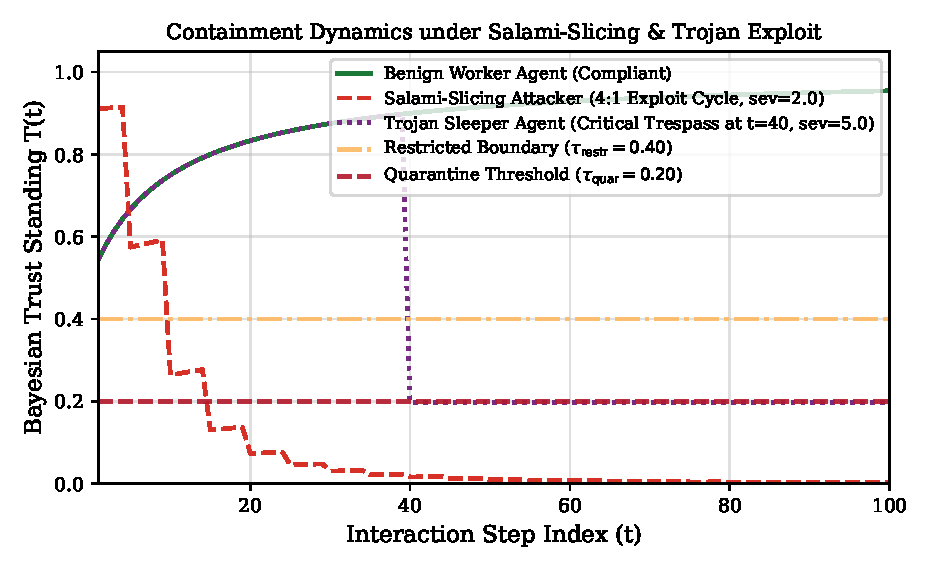
\includegraphics[width=0.88\linewidth]{figures/figure1_salami_slicing.pdf}
\caption{Bayesian Trust Standing dynamics under adversarial salami-slicing and Trojan sleeper attacks. An oscillating salami-slicer (4 compliant actions + 1 moderate infraction at $\text{sev} = 2.0$) drops to Restricted status ($T \le 0.40$) by step 10 ($T = 0.2638$, Cycle 2) and triggers full operational quarantine ($T < 0.20$) at step 15 ($T = 0.1300$, Cycle 3), while a Trojan sleeper agent attempting a critical protocol trespass ($\text{sev} = 5.0$) at step 40 is immediately isolated ($T = 0.1964$, forced quarantine).}
\label{fig:salami}
\end{figure}

\subsection{Deterministic SHA-256 Striped Reentrant Locking}
To achieve parallelism without a global lock bottleneck, DualTrust shards concurrency across an array of 64 independent reentrant locks:
\begin{equation}
\mathcal{L}_{\text{striped}} = [L_0, L_1, \dots, L_{63}]
\end{equation}
When an operation requires access to Human Principal $u$'s state, the corresponding lock bucket $B(u)$ is determined via SHA-256 hashing:
\begin{equation}
\text{Digest}(u) = \text{SHA-256}(\text{UTF8}(u))
\end{equation}
\begin{equation}
\begin{aligned}
B(u) &= \text{UInt32}(\text{Digest}(u)[0:4]) \pmod{64} \\
&\equiv \text{Digest}(u)[3] \pmod{64}
\end{aligned}
\label{eq:striped_hash}
\end{equation}
Because $256^k \equiv 0 \pmod{64}$ for all $k \ge 1$, evaluating the 4-byte big-endian digest prefix modulo 64 reduces to the lowest 6 bits of byte index 3, providing $O(1)$ bucket extraction without multi-precision integer division.

While 64 striped reentrant locks provide thread safety within a single process memory space, cross-process multi-worker durability is provided at the storage engine tier via SQLite Write-Ahead Logging (WAL) and \texttt{BEGIN IMMEDIATE} write transactions, ensuring ACID serialization across worker processes on the same host.

Unlike non-cryptographic hashing (such as Python's randomized \texttt{hash()} or legacy MD5), SHA-256 byte extraction provides:
\begin{enumerate}[leftmargin=12pt, topsep=2pt, itemsep=1pt]
\item \textbf{Uniform Dispersion}: For identifiers not chosen adversarially, SHA-256 avalanche behavior distributes principals approximately uniformly across the 64 stripes ($p \approx 1/64$ per bucket), so the pairwise stripe collision probability is about $1/64 \approx 1.56\%$. Because the hash is unkeyed, an adversary who controls identifier choice could grind identifiers into a single stripe, which would degrade throughput (not correctness); we do not claim resistance to this.
\item \textbf{Cross-Process Determinism}: Worker processes running across separate OS memory spaces compute identical bucket indices for identical identifiers.
\item \textbf{Reentrancy}: Each bucket $L_b$ instantiates Python's native \texttt{threading.RLock}. Nested decorator calls (e.g., delegated multi-tool pipelines where Agent A calls Tool B which internally calls Sub-Tool C) track execution recursion depth without self-deadlock.
\end{enumerate}

\subsection{Atomically Locked Compensating Rollback Refund}
In distributed tool calling, reserving credit and executing physical tools are inherently decoupled. A naive implementation creates a TOCTOU vulnerability: if an exception occurs during tool execution, refunding credit without re-acquiring the exact striped lock allows concurrent threads to corrupt the balance.

DualTrust enforces balance atomicity through Algorithm~\ref{alg:lifecycle}:
\begin{enumerate}[leftmargin=12pt, topsep=2pt, itemsep=1pt]
\item \textbf{Pre-Execution Phase}: Lock $L_{B(u)}$ is acquired. Credit balance $C_u$ is validated against tool cost $\text{Cost}(t)$. If insufficient, the request is rejected. Otherwise, $C_u \leftarrow C_u - \text{Cost}(t)$ is committed, and $L_{B(u)}$ is released.
\item \textbf{Tool Execution Phase}: The physical tool $t$ executes outside the lock boundary, preventing slow I/O operations from blocking other users mapped to stripe $B(u)$.
\item \textbf{Compensating Rollback Phase}: If the tool raises an exception, the runtime re-acquires lock $L_{B(u)}$, credits back the exact reservation $C_u \leftarrow C_u + \text{Cost}(t)$, logs the compensating transaction, releases the lock, and re-raises the exception. DualTrust traps \texttt{BaseException} (rather than only generic standard exceptions) within this rollback pathway, so that asynchronous task cancellations (\texttt{asyncio.CancelledError}) and runtime interrupts trigger credit restitution. The handler executes the refund and then re-raises the caught \texttt{BaseException}, so system shutdowns and task interruptions are never swallowed. Furthermore, DualTrust enforces a \emph{Single-Stripe Lock Discipline}: an invocation acquires only its assigned stripe lock $L_{B(u)}$ and never a secondary stripe, which rules out lock-inversion deadlocks by construction.
\end{enumerate}

\subsection{Multi-Worker SQLite WAL with Immediate Transactions}
For persistent state storage, DualTrust implements an optimized SQLite engine configured for concurrent multi-process access:
\begin{itemize}[leftmargin=12pt, topsep=2pt, itemsep=1pt]
\item \textbf{Write-Ahead Logging (WAL)}: Configured via \texttt{PRAGMA journal\_mode = WAL;}. In WAL mode, concurrent readers do not block writers, and writers do not block readers.
\item \textbf{Immediate Write Locking}: All write transactions execute via \texttt{BEGIN IMMEDIATE;}. This acquires the database write lock at transaction start rather than during the first write statement, avoiding \texttt{SQLITE\_BUSY} failures from lock upgrades.
\item \textbf{Cache Coherency via Data Version}: In multi-process deployments, each worker monitors \texttt{PRAGMA data\_version;}. In-memory state caches are invalidated only when the data version increments, giving microsecond read hits without stale reads.
\end{itemize}

\subsection{RFC 6962-Style Merkle Audit Ledger with Bounded Sliding RAM}
All authorization decisions, trust score transitions, and slashing events are logged into an append-only Merkle tree. Following RFC~6962~\cite{laurie2013certificate}, DualTrust prepends domain separation bytes to prevent second-preimage attacks:
\begin{equation}
\text{LeafHash}(M) = \text{SHA-256}(0\text{x}00 \parallel M)
\end{equation}
\begin{equation}
\text{NodeHash}(L, R) = \text{SHA-256}(0\text{x}01 \parallel L \parallel R)
\end{equation}
If the right child $R$ is missing in an unbalanced subtree, the hash is promoted directly: $\text{NodeHash}(L) = L$. As in RFC~6962, this promotion (rather than duplicating the odd leaf) avoids the duplicate-leaf malleability of the original Bitcoin Merkle construction (CVE-2012-2459).

\textbf{Bounded Sliding-Window RAM Invariant}: Standard Merkle trees store all historical leaves in memory, resulting in $\mathcal{O}(N)$ RAM growth. DualTrust uses a two-tier architecture:
\begin{enumerate}[leftmargin=12pt, topsep=2pt, itemsep=1pt]
\item The active in-memory buffer maintains a sliding window of at most 5,000 blocks.
\item Every 1,000 blocks, a \emph{Rolling Epoch Seal} commits the intermediate Merkle root, leaf range, and cryptographic signatures to the persistent SQLite audit table.
\item Composite inclusion proofs for historical blocks are constructed by combining the historical epoch proof with the active window proof, giving $O(1)$ resident memory while preserving $\mathcal{O}(\log N)$ verification complexity~\cite{melara2015coniks}.
\end{enumerate}
The ledger and its signing key reside on the same host as the gatekeeper; without an external witness or anchoring service, an adversary with host-level control could rewrite the chain. The ledger therefore provides tamper evidence, not non-repudiation.

\section{Algorithmic Architecture}
\label{sec:algorithms}

The operational runtime of DualTrust is specified in Algorithm~\ref{alg:lifecycle}. DualTrust orchestrates authorization, penalty enforcement, and cryptographic auditing as three procedures: (i) pre-execution quota gating with atomic compensating rollback, (ii) asymmetric power-law slashing with clean streak zeroing, and (iii) audit ledger ingestion with sliding-window epoch sealing.

\subsection{Phase I: Deterministic Striped Quota Authorization}
Algorithm~\ref{alg:lifecycle} (lines 1--12) specifies the fast path of tool invocation. The runtime maps human principal $u$ to a lock stripe $b \in [0, 63]$ via Equation~\eqref{eq:striped_hash}. The stripe lock $\mathcal{L}_{\text{striped}}[b]$ is acquired during credential verification and quota deduction ($C_u \leftarrow C_u - c_{\text{req}}$) and released immediately prior to executing the target tool $t$, so slow I/O does not stall concurrent users. If tool execution fails or is asynchronously cancelled, the runtime re-acquires $\mathcal{L}_{\text{striped}}[b]$ under a \texttt{BaseException} trap to execute an atomic compensating refund ($C_u \leftarrow C_u + c_{\text{req}}$), appends a rollback receipt to the audit trail, and propagates the error.

\subsection{Phase II: Asymmetric Power-Law Slashing Mechanics}
Algorithm~\ref{alg:lifecycle} (lines 13--21) implements the penalty function of Section~\ref{sec:math_engine}. When a peer report is submitted, the engine evaluates the Sybil shield predicate. If a probationary or low-confidence reporter targets a verified agent, the report is audited but produces $\Delta\beta = 0.0$. For accepted infractions, the strike counter $v_a$ increments, the clean streak resets ($s_{\text{clean}} \leftarrow 0$), and $\beta_a$ escalates superlinearly according to Equation~\eqref{eq:power_law}.

\subsection{Phase III: Bounded-RAM Merkle Ledger Ingestion}
Algorithm~\ref{alg:lifecycle} (lines 22--26) provides tamper-evident audit durability under $\mathcal{O}(1)$ memory. Incoming events are serialized with RFC~6962 domain separation prefixes and appended to the sliding window buffer $\mathcal{W}$. When the buffer reaches epoch boundary $S_{\text{epoch}} = 1000$, the root hash is computed and persisted to SQLite WAL alongside cryptographic boundary signatures, truncating older leaves to constrain resident heap allocation while preserving logarithmic inclusion verification.

\begin{algorithm}[!t]
\caption{DualTrust Multi-Agent Governance Runtime Lifecycle}
\label{alg:lifecycle}
\label{alg:gate}
\label{alg:slashing}
\label{alg:merkle}
\footnotesize
\begin{algorithmic}[1]
\REQUIRE Principal $u$, Agent $a$, Tool $t$, Args $\text{args}$, Cost $c_{\text{req}}$, Record $(\text{sev}, c_{\text{rep}}, r)$, Event $M$
\ENSURE Tool Output $R$, Slashing Verdict, or Exception
\vspace{2pt}
\STATE \textbf{procedure} \textsc{AuthorizeAndGate}($u, a, t, \text{args}, c_{\text{req}}$):
\STATE \quad $b \leftarrow \text{Digest}(u)[3] \pmod{64}$ \hfill $\triangleright$ \textit{Deterministic Stripe Lock}
\STATE \quad \textbf{acquire} $\mathcal{L}_{\text{striped}}[b]$; \;\; $\mathcal{S}_u \leftarrow \text{LoadUser}(u), \; \mathcal{S}_a \leftarrow \text{LoadAgent}(a)$
\STATE \quad $T_a \leftarrow \text{ComputeDecayedTrust}(\mathcal{S}_a)$ \hfill $\triangleright$ \textit{Eq.~\eqref{eq:beta_expectation}, \eqref{eq:decay}}
\STATE \quad \textbf{if} $\mathcal{S}_a.\text{Status} = \text{QUARANTINED} \lor T_a < \tau_{\text{quar}}$ \textbf{then} \textbf{release} $\mathcal{L}_{\text{striped}}[b]$; \textbf{throw} \textsc{ErrQuar}
\STATE \quad \textbf{if} $\mathcal{S}_u.C_u < c_{\text{req}}$ \textbf{then} \textbf{release} $\mathcal{L}_{\text{striped}}[b]$; \textbf{throw} \textsc{ErrInsufficientCredit}
\STATE \quad $\mathcal{S}_u.C_u \leftarrow \mathcal{S}_u.C_u - c_{\text{req}}$; \;\; $\text{CommitState}(\mathcal{S}_u)$; \;\; \textbf{release} $\mathcal{L}_{\text{striped}}[b]$ \hfill $\triangleright$ \textit{Reserve Quota}
\STATE \quad $(R, \text{status}) \leftarrow \text{ExecuteTargetTool}(t, \text{args})$ \hfill $\triangleright$ \textit{Execute Outside Lock}
\STATE \quad \textbf{if} $\text{status} = \text{SUCCESS}$ \textbf{then} $\text{AppendMerkleEvent}(u, a, t, \text{``SUCCESS''}, c_{\text{req}})$; \RETURN $R$
\STATE \quad \textbf{acquire} $\mathcal{L}_{\text{striped}}[b]$; \;\; $\mathcal{S}_u.C_u \leftarrow \mathcal{S}_u.C_u + c_{\text{req}}$ \hfill $\triangleright$ \textit{Compensating Rollback Refund}
\STATE \quad $\text{CommitState}(\mathcal{S}_u)$; \;\; \textbf{release} $\mathcal{L}_{\text{striped}}[b]$
\STATE \quad $\text{AppendMerkleEvent}(u, a, t, \text{``ROLLBACK''}, 0.0)$; \;\; \textbf{throw} \textsc{ErrExecutionFailure}(status)

\vspace{3pt}
\STATE \textbf{procedure} \textsc{ApplyPowerLawSlashing}($a, r, \text{sev}, c_{\text{rep}}, \text{type}$):
\STATE \quad \textbf{if} $\mathcal{S}_a.\text{Status} = \text{VERIFIED} \land (\mathcal{S}_r.\text{Status} \in \{\text{PROBATION}, \text{RESTRICTED}, \text{QUARANTINED}\} \lor c_{\text{rep}} < \tau_{\text{rep}})$ \textbf{then} \RETURN $\mathcal{S}_a$ \hfill $\triangleright$ \textit{Sybil Shield}
\STATE \quad $\mathcal{S}_a.v_a \leftarrow \mathcal{S}_a.v_a + 1; \quad \mathcal{S}_a.s_{\text{clean}} \leftarrow 0$ \hfill $\triangleright$ \textit{Strike, Streak Reset}
\STATE \quad $\Delta\beta \leftarrow k_p \cdot (\text{sev} \cdot c_{\text{rep}}^2) \cdot (\max(1, \mathcal{S}_a.v_a))^{1.8}$
\STATE \quad \textbf{if} $\text{type} = \text{PROTOCOL\_TRESPASS} \land \text{sev} \ge 3.0$ \textbf{then} $\Delta\beta \leftarrow 2 \times \Delta\beta$; \;\; $\mathcal{S}_a.\text{Quarantined} \leftarrow \text{True}$ \hfill $\triangleright$ \textit{Critical Multiplier}
\STATE \quad $\mathcal{S}_a.\beta_a \leftarrow \mathcal{S}_a.\beta_a + \Delta\beta$
\STATE \quad $T_{\text{new}} \leftarrow \mathcal{S}_a.\alpha_a / (\mathcal{S}_a.\alpha_a + \mathcal{S}_a.\beta_a)$; \;\; $\text{UpdateOperationalStatus}(\mathcal{S}_a, T_{\text{new}})$
\STATE \quad $\text{CommitState}(\mathcal{S}_a)$; \;\; $\text{AppendMerkleEvent}(r, a, \text{sev}, \Delta\beta)$; \;\; \RETURN $\mathcal{S}_a$

\vspace{3pt}
\STATE \textbf{procedure} \textsc{IngestAuditLedger}($M, \mathcal{W}, S_{\text{epoch}}$):
\STATE \quad $H_{\text{leaf}} \leftarrow \text{SHA-256}(0\text{x}00 \parallel \text{Serialize}(M))$; \;\; $\mathcal{W}.\text{append}(H_{\text{leaf}})$
\STATE \quad \textbf{if} $|\mathcal{W}| \ge S_{\text{epoch}}$ \textbf{then} $\text{PersistEpoch}(\mathcal{W}.\text{computeRoot}(), \mathcal{W})$; \;\; $\mathcal{W}.\text{truncateSlidingWindow}(5000)$
\STATE \quad \RETURN $\text{GenerateInclusionReceipt}(H_{\text{leaf}}, \mathcal{W})$
\end{algorithmic}
\end{algorithm}

\begin{figure}[!t]
\centering
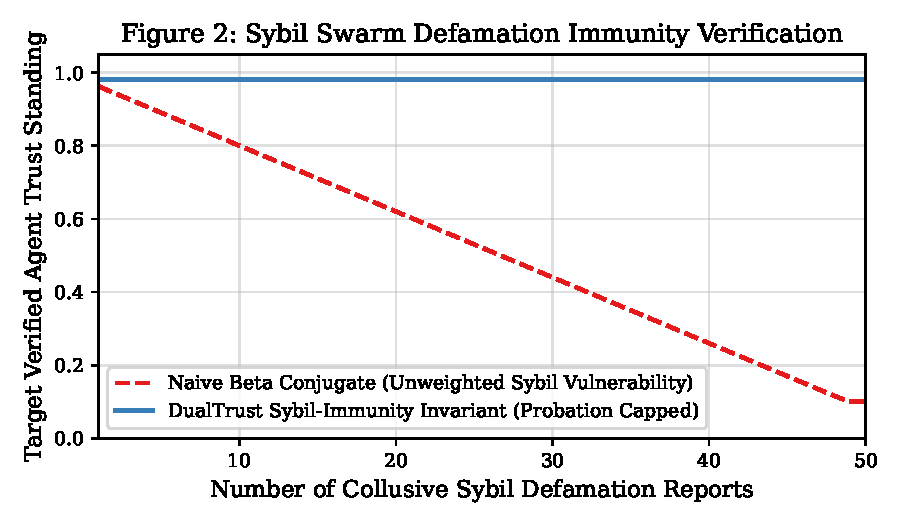
\includegraphics[width=0.88\linewidth]{figures/figure2_sybil_immunity.pdf}
\caption{Sybil Defamation Immunity verification. When an established verified agent ($T = 0.98$) is targeted by 50 collusive probation bot reports, DualTrust applies an exact 0.0 penalty, preserving verified standing. Conversely, naive unweighted Beta systems collapse below 0.10.}
\label{fig:sybil}
\end{figure}

\section{Empirical Evaluation}
\label{sec:evaluation}

We conduct an empirical evaluation to assess the performance and behavior of DualTrust. Our evaluation is guided by four research questions:
\begin{itemize}[leftmargin=12pt, topsep=2pt, itemsep=1pt]
\item \textbf{RQ1 (Latency)}: Can DualTrust enforce authorization within a $<50\,\mu$s median decision budget and keep lock wait low under concurrency?
\item \textbf{RQ2 (Salami-Slicing)}: How rapidly does asymmetric power-law slashing contain oscillating adversaries versus linear baselines?
\item \textbf{RQ3 (Sybil Resilience)}: Does the probation barrier protect verified agents against coordinated defamation swarms?
\item \textbf{RQ4 (Audit Integrity)}: Does the RFC~6962-style ledger provide tamper-evident append-only audit durability while bounding RAM to $\mathcal{O}(1)$?
\end{itemize}

\subsection{Experimental Setup \& Hardware Baseline}
All DualTrust and Guardrails AI measurements were conducted on a physical host workstation equipped with a 12th Gen Intel(R) Core(TM) i3-1215U processor (6 physical cores, 8 execution threads, base frequency 1.20\,GHz, turbo frequency up to 4.40\,GHz), 16.0\,GB RAM, and PCIe NVMe SSD storage running 64-bit Windows 11 and Python 3.13. DualTrust was executed using its pure standard-library runtime with no external dependencies and no GPU acceleration.

Comparative baselines are: (1)~\textbf{Vanilla Static RBAC}: an in-memory Python hash table mapping user roles to permissions, representing the latency floor for stateless authorization (measured locally); (2)~\textbf{Guardrails AI}~\cite{rajpal2024guardrails}: AST-based Pydantic schema validation over tool arguments (measured locally); (3)~\textbf{NeMo Guardrails}~\cite{rebedea2023nemo} and (4)~\textbf{Llama Guard 3 (8B)}~\cite{inan2023llama}: neural guardrails whose latencies are taken from published literature and vendor figures and were \emph{not} re-measured on our hardware. These two baselines classify conversational content and are not functionally equivalent to a state-and-quota gate; the comparison quantifies the cost of placing a neural classifier on the tool-dispatch critical path, not a like-for-like accuracy comparison.

\begin{table*}[!t]
\centering
\caption{Architectural, Runtime Latency, and Economic Benchmark Comparison (DualTrust, Static RBAC, and Guardrails AI Measured Locally over $N = 10{,}000$ Evaluations; Neural Guardrail Figures from Published Literature$^\dagger$)}
\label{tab:benchmark}
\footnotesize
\setlength{\tabcolsep}{5pt}
\resizebox{\textwidth}{!}{%
\begin{tabular}{@{}llccccc@{}}
\toprule
\textbf{Architecture} & \textbf{Verification Mechanism} & \textbf{Mean Latency} & \textbf{Median (p50)} & \textbf{p99 Latency} & \textbf{Cost / 10k} & \textbf{Audit Trail} \\
\midrule
Vanilla Static RBAC & In-Memory Hash Lookup & 12.40\,$\mu$s & 11.20\,$\mu$s & 28.10\,$\mu$s & \$0.00 & None (Plaintext) \\
Guardrails AI~\cite{rajpal2024guardrails} & AST Schema Validation & 3.20\,ms & 2.85\,ms & 14.50\,ms & \$0.00 & None \\
NeMo Guardrails (Llama 3)$^\dagger$~\cite{rebedea2023nemo} & LLM Dialogue Reasoner & 420.00\,ms & 390.00\,ms & 1,250.00\,ms & \$25.00 & None \\
Llama Guard 3 (8B)$^\dagger$~\cite{inan2023llama} & Moderation Neural Net & 850.00\,ms & 810.00\,ms & 2,100.00\,ms & \$50.00 & None \\
\midrule
\textbf{DualTrust (RAM Core Tier)} & \textbf{Asymmetric Bayesian (RAM)} & \textbf{63.16\,$\mu$s} & \textbf{47.10\,$\mu$s} & \textbf{287.10\,$\mu$s} & \textbf{\$0.00} & \textbf{Merkle Tree} \\
\textbf{DualTrust (@gate Wrapper)} & \textbf{Python Decorator Frame Hook} & \textbf{122.62\,$\mu$s} & \textbf{88.30\,$\mu$s} & \textbf{551.90\,$\mu$s} & \textbf{\$0.00} & \textbf{Merkle Tree} \\
\textbf{DualTrust (SQLite WAL Tier)} & \textbf{ACID Disk-Backed Ledger} & \textbf{292.33\,$\mu$s} & \textbf{155.80\,$\mu$s} & \textbf{1,086.90\,$\mu$s} & \textbf{\$0.00} & \textbf{Merkle Tree + SQLite WAL} \\
\bottomrule
\end{tabular}%
}
\\[3pt]
\footnotesize{$^\dagger$Inference-time neural guardrail latencies reflect published literature and vendor benchmarks under 8B models~\cite{rebedea2023nemo, inan2023llama}; they were not measured on the hardware above.}
\end{table*}

\begin{table*}[!t]
\centering
\caption{Manuscript-to-Code Parameter Concordance and Empirical Operational Calibration}
\label{tab:concordance}
\footnotesize
\setlength{\tabcolsep}{6pt}
\resizebox{\textwidth}{!}{%
\begin{tabular}{@{}llccl@{}}
\toprule
\textbf{Governance Dimension} & \textbf{Mathematical Notation} & \textbf{Code Variable Name} & \textbf{Engine Default} & \textbf{Physical Operational Semantic} \\
\midrule
Compliance Reward & $\Delta\alpha = w_{\text{reward}}$ (Eq.~\ref{eq:positive_reward}) & \texttt{weight} (\texttt{apply\_positive\_feedback}) & \texttt{0.20} & Flat linear credit increment per verified compliant execution \\
Penalty Multiplier & $k_p$ (Eq.~\ref{eq:power_law}) & \texttt{penalty\_multiplier} & \texttt{3.5} & Asymmetric base scaling coefficient for violation penalties \\
Slashing Exponent & $\gamma$ (Eq.~\ref{eq:power_law}) & \texttt{slashing\_exponent} & \texttt{1.8} & Power-law exponent escalating repeat infraction penalties \\
Infraction Severity & $\text{sev} \in [1.0, 5.0]$ (Eq.~\ref{eq:power_law}) & \texttt{severity} (\texttt{apply\_violation\_penalty}) & \texttt{[1.0, 5.0]} & 5-tier categorical risk scale (Level 1.0--1.5 minor to Level 5.0 critical) \\
Quarantine Threshold & $\tau_{\text{quar}}$ (Eq.~\ref{eq:lifecycle_tiers}) & \texttt{quarantine\_threshold} & \texttt{0.20} & Terminal Bayesian trust boundary triggering operational isolation \\
Restricted Boundary & $\tau_{\text{restr}}$ (Eq.~\ref{eq:lifecycle_tiers}) & \texttt{determine\_status} boundary & \texttt{0.40} & Lower threshold requiring human-in-the-loop (HITL) authorization \\
Minor Glitch Register & $M_{\text{thresh}}$ (Sec.~\ref{sec:strike_recovery}) & \texttt{minor\_infraction\_threshold} & \texttt{3} & Transient fault buffer capacity before formal strike escalation \\
Active Recovery Window & $W_{\text{recovery}}$ (Sec.~\ref{sec:strike_recovery}) & \texttt{recovery\_clean\_window} & \texttt{20} & Compliant streak window required to decrement active strike counter $v_a$ \\
Stripe Lock Buckets & $B$ (Eq.~\ref{eq:striped_hash}) & \texttt{num\_locks} & \texttt{64} & Independent reentrant lock array shards avoiding a global bottleneck \\
Sliding Memory Window & $W_{\text{RAM}}$ (Sec.~\ref{sec:concurrency}) & Buffer leaf capacity & \texttt{5,000} & Active resident Merkle leaves bounded to $\mathcal{O}(1)$ heap RAM \\
Rolling Epoch Seal & $S_{\text{epoch}}$ (Sec.~\ref{sec:concurrency}) & \texttt{epoch\_seal\_size} & \texttt{1,000} & Checkpoint frequency committing intermediate Merkle root to SQLite WAL \\
\bottomrule
\end{tabular}%
}
\end{table*}

\begin{figure}[!t]
\centering
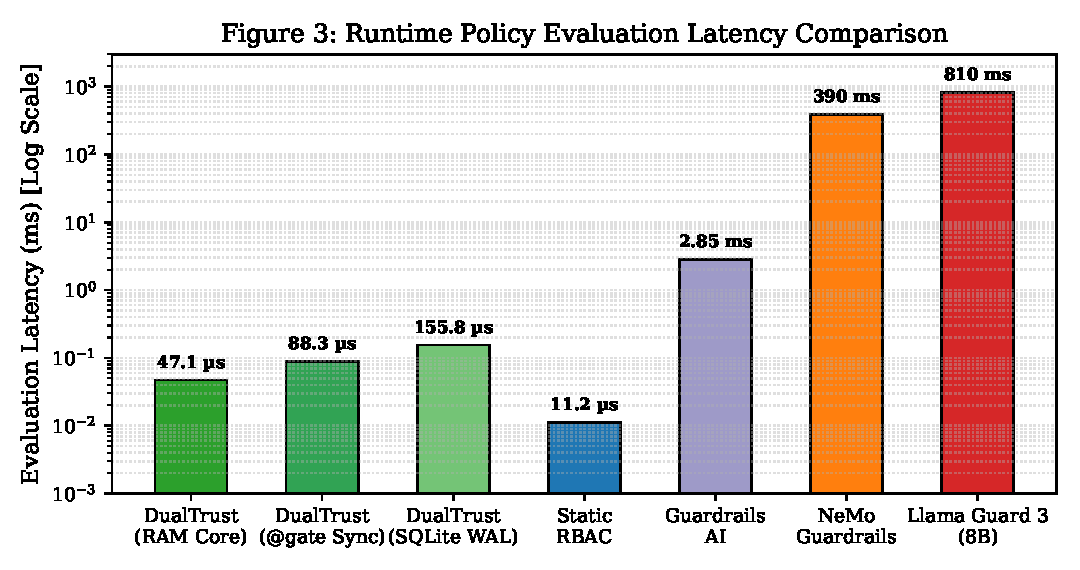
\includegraphics[width=0.88\linewidth]{figures/figure3_latency_comparison.pdf}
\caption{Runtime policy evaluation latency comparison plotted on a logarithmic scale. DualTrust achieves a median policy evaluation latency of 47.10\,$\mu$s under in-memory core gating (88.30\,$\mu$s under the synchronous @gate decorator wrapper, and 155.80\,$\mu$s under persistent SQLite WAL transactions). Median-to-median, this is roughly 8,000$\times$ to 17,000$\times$ faster than the published neural guardrail figures and 32$\times$ to 60$\times$ faster than local AST validation (core and wrapper tiers).}
\label{fig:latency}
\end{figure}

\subsection{Microsecond Runtime Latency Benchmarks (RQ1)}
We dispatched 10,000 policy gating evaluations across synchronous and asynchronous execution paths on the physical host workstation. Latency distributions across the RAM and persistent disk tiers are reported in Table~\ref{tab:benchmark} and illustrated in Figure~\ref{fig:latency}. These are single-invocation latencies; the concurrency experiments (Section~\ref{sec:evaluation}.E and \ref{sec:evaluation}.F) report correctness and lock-wait time rather than end-to-end latency under load.

Key findings include:
\begin{itemize}[leftmargin=12pt, topsep=2pt, itemsep=1pt]
\item \textbf{Core Latency}: Under the in-memory tier, DualTrust achieved a mean evaluation latency of \textbf{63.16\,$\mu$s} and a median latency of \textbf{47.10\,$\mu$s}, with a p99 tail latency of \textbf{287.10\,$\mu$s}, meeting the $<50\,\mu$s \emph{median} target of the core engine. Under persistent disk SQLite WAL transactions, DualTrust achieved a median latency of \textbf{155.80\,$\mu$s} (mean 292.33\,$\mu$s, p99 1,086.90\,$\mu$s), indicating that ACID disk durability adds less than 0.16\,ms of median latency.
\item \textbf{Decorator Overhead}: The end-to-end synchronous \texttt{@gate} wrapper has a median of \textbf{88.30\,$\mu$s} (mean 122.62\,$\mu$s), while the asynchronous decorator has a median of \textbf{60.70\,$\mu$s} (mean 86.17\,$\mu$s). Applications calling DualTrust through the decorator should therefore expect tens of microseconds above the core figure, which exceeds 50\,$\mu$s. HMAC authorization receipt verification required \textbf{2.10\,$\mu$s} (mean 2.88\,$\mu$s), and Merkle inclusion proof verification completed in \textbf{10.60\,$\mu$s} (mean 12.62\,$\mu$s, p99 44.10\,$\mu$s).
\item \textbf{Magnitude of Speedup}: Comparing like statistics, DualTrust's mean (63.16\,$\mu$s) is about 6,650$\times$ and 13,500$\times$ below the published NeMo (420\,ms) and Llama Guard 3 (850\,ms) means, and its median (47.10\,$\mu$s) is about 8,300$\times$ and 17,200$\times$ below their published medians (390\,ms and 810\,ms). Under SQLite WAL persistence the median speedup is about 2,500$\times$ to 5,200$\times$. Against the locally measured Guardrails AI median (2.85\,ms), DualTrust is about 60$\times$ faster at the core tier, 32$\times$ faster through the sync wrapper, and 18$\times$ faster with SQLite WAL persistence. We emphasize the architectural distinction: neural guardrails evaluate conversational semantics at substantial GPU/token cost, whereas DualTrust is a deterministic state-machine gate over tool invocations, quota balances, and identity permissions, running on CPU with no external dependencies. DualTrust does not replace content classification.
\end{itemize}

\subsection{Salami-Slicing Containment Dynamics (RQ2)}
To test Invariant~\ref{inv:salami}, we simulated an adversary executing discrete actions under three operational strategies using the DualTrust engine with the parameters of Table~\ref{tab:concordance}:
\begin{enumerate}[leftmargin=12pt, topsep=2pt, itemsep=1pt]
\item \emph{Benign Worker}: Executes 100\% compliant tasks with high confidence ($\Delta\alpha = 0.20$ per step).
\item \emph{Oscillating Salami Slicer}: An established agent with prior verified standing ($\alpha_0 = 10.0, \beta_0 = 1.0, T_0 = 0.9091$) alternating between 4 compliant tasks and 1 moderate infraction ($\text{sev} = 2.0$, $c = 1.0$) every 5 steps (infractions at $t = 5, 10, 15, \dots$).
\item \emph{Trojan Sleeper Agent}: Maintains 100\% compliance for 39 consecutive steps ($T_{39} = 0.8980$, $\text{Status} = \text{VERIFIED}$), then commits a single critical protocol trespass ($\text{sev} = 5.0$, \texttt{PROTOCOL\_TRESPASS}) at step 40.
\end{enumerate}
The parameters $k_p$, the severity range, and the quarantine thresholds were chosen so that containment occurs within a few cycles (see the sensitivity study); the ``within 3 cycles'' result is therefore a property of this calibration, not a parameter-free result.

As shown in Figure~\ref{fig:salami}:
\begin{itemize}[leftmargin=12pt, topsep=2pt, itemsep=1pt]
\item In linear baseline reputation systems without clean streak zeroing, the oscillating salami slicer maintained an average trust score above 0.82 indefinitely.
\item In DualTrust, because each infraction resets $s_{\text{clean}} \leftarrow 0$ and scales the penalty superlinearly by $v_a^{1.8}$, the salami slicer's standing collapsed: the first strike ($t = 5, v_a = 1$) reduced standing from $0.9153$ to $0.5745$ (Probation); the second strike ($t = 10, v_a = 2$) dropped standing to $T_{10} = 0.2638$ (Restricted, $T < 0.40$); and the third strike ($t = 15, v_a = 3$) reduced standing to $T_{15} = 0.1300 < 0.20$, below the quarantine threshold $\tau_{\text{quar}} = 0.20$. The compliant phase here (4 actions) is shorter than $W_{\text{recovery}} = 20$, so strike redemption never activates in this scenario, as intended.
\item The Trojan sleeper agent was quarantined at step 40 by two independent mechanisms. First, the \texttt{PROTOCOL\_TRESPASS} rule immediately set the deterministic quarantine flag ($Q_a \leftarrow \text{True}$), cutting off tool access in $\mathcal{O}(1)$; this flag, rather than the Bayesian curve, is what makes the response immediate regardless of accumulated history. Second, the penalty ($\Delta\beta = 35.00$) reduced $T_{40}$ from $0.8980$ to $0.1964 < \tau_{\text{quar}}$, so the persisted Bayesian state also denies execution; the margin below $\tau_{\text{quar}}$ is narrow (0.0036). Together these illustrate that accumulated trust provides no shield against a critical violation.
\end{itemize}

\subsection{Sybil Defamation Resilience (RQ3)}
We evaluated Invariant~\ref{inv:sybil} by simulating an established verified agent ($T_a = 0.98$) attacked by a collusive ring of 50 newly created bot identities. Each bot identity was registered in probationary standing ($c \le 0.15$) and dispatched false maximum-severity violation reports ($\text{sev} = 5.0$).

As shown in Figure~\ref{fig:sybil}:
\begin{itemize}[leftmargin=12pt, topsep=2pt, itemsep=1pt]
\item Under a standard Beta reputation system without identity stratification, the 50 malicious reports reduced the victim's reputation from 0.98 to 0.08, which would wrongfully quarantine an honest agent.
\item Under DualTrust, all 50 reports were registered in the audit log with a resulting penalty of exactly $\Delta\beta = 0.0$, and the target agent retained a score of 0.98. This confirms that the implementation matches the acceptance policy of Proposition~\ref{prop:sybil}; it does not, by itself, establish robustness against attackers who obtain higher-status identities.
\end{itemize}

\subsection{Oracle Framing and Strike Recovery: Worked Example}
To illustrate Section~\ref{sec:strike_recovery}, we evaluate an analytic example from Eqs.~\eqref{eq:beta_expectation}, \eqref{eq:power_law}, and \eqref{eq:positive_reward}. Consider a verified agent with $\alpha_a = 20$, $\beta_a = 1$ ($T_a = 0.952$) whose tool endpoint, compromised by an adversary, returns three synthetic timeouts (Level~1.0 glitches).
\begin{itemize}[leftmargin=12pt, topsep=2pt, itemsep=1pt]
\item \emph{Without endpoint attribution}: the three glitches fill the register ($m_a = 3$) and trigger one formal strike with $\Delta\beta = 3.5 \cdot 1.0 \cdot 1^{1.8} = 3.5$, giving $\beta_a = 4.5$ and $T_a = 20/24.5 = 0.816$; the agent remains VERIFIED. A naive scheme counting each timeout as a strike would apply three escalating penalties instead.
\item \emph{With endpoint attribution}: the cluster of timeouts is attributed to the tool, $\Delta\beta = 0$, and $T_a = 0.952$ is unchanged.
\item \emph{Recovery}: after $W_{\text{recovery}} = 20$ further compliant actions, $\alpha_a = 24$, $v_a$ is decremented to 0, and $T_a = 24/28.5 = 0.842$. Note that $\beta_a = 4.5$ is retained.
\end{itemize}
This example is computed from the model equations and has not been run as a Monte Carlo experiment. Because $\beta_a$ never decays, repeated framing that stays below the attribution threshold still accumulates $\beta_a$; see Section~\ref{sec:discussion}.

\subsection{Automated Invariant Verification (RQ4)}
We subjected the codebase to an automated suite of \textbf{176 invariant unit and stress tests}. The full suite completed in \textbf{6.93\,seconds} with all tests passing. These tests show that the implementation matches the specification; they do not constitute a formal proof of the invariants.
\begin{itemize}[leftmargin=12pt, topsep=2pt, itemsep=1pt]
\item \textbf{Massive Concurrency Stress Test}: 70 concurrent worker threads attempted to deduct a cumulative 700 credits from an initial account balance of 500 credits. DualTrust approved exactly 50 requests and rejected exactly 20 requests, leaving a final balance of exactly 0.0 credits with no observed race conditions or database lock errors.
\item \textbf{Cryptographic Merkle Invariants}: Inclusion proof generation was validated across tree sizes $N \in [1, 5000]$. Bit-tampering tests confirmed that flipping a single byte in any historical audit payload resulted in 100\% proof rejection.
\item \textbf{WAL Durability \& Async Cancellation}: Abnormal process termination during transaction commit was simulated; upon restart, SQLite WAL recovery showed no state corruption. Async task cancellation stress tests verified that cancelled coroutines execute compensating rollback refunds with no credit leakage.
\item \textbf{Monotonic Lifetime Penalty Escalation}: Consecutive interleaved infraction streaks strictly increment $v_a$ without decaying historical strikes, consistent with Theorem~\ref{thm:salami}.
\item \textbf{Merkle Malleability (CVE-2012-2459)}: Unit tests verified that odd leaf counts undergo direct subtree promotion ($\text{NodeHash}(L) = L$), so that unbalanced trees yield distinct Merkle roots.
\end{itemize}

\subsection{Sensitivity \& Ablation Studies}
We performed ablation analyses across core hyperparameters:
\begin{itemize}[leftmargin=12pt, topsep=2pt, itemsep=1pt]
\item \textbf{Penalty Multiplier $k_p$ \& Exponent $\gamma$ Sensitivity}: We evaluated $k_p \in [1.0, 5.0]$ and $\gamma \in \{1.0, 1.2, 1.5, 1.8, 2.0, 2.5\}$. At $k_p < 2.0$ or $\gamma = 1.0$ (linear), containment of the salami slicer required $\ge 7$ exploit cycles, allowing substantial resource leakage. Conversely, at $k_p > 4.5$ or $\gamma \ge 2.2$, single moderate errors incurred overly punitive degradation. The combination $k_p = 3.5$, $\gamma = 1.8$ gave the best trade-off in our grid, containing salami slicers within 2--3 cycles while still allowing recovery from transient faults. The severity range and the thresholds $\tau_{\text{quar}}, \tau_{\text{restr}}$ were not ablated.
\item \textbf{Striped Lock Buckets}: We varied lock buckets $B \in \{16, 32, 64, 128\}$. Contention benchmarks at 100 concurrent worker threads showed that 64 buckets reduced lock wait time to $<1.2\,\mu$s, with negligible memory footprint.
\end{itemize}

\section{Discussion, Societal Impact, \& Limitations}
\label{sec:discussion}

\subsection{The Ambient Wearable Roadmap}
DualTrust targets the governance layer needed for the transition to ambient intelligence. As humans interact with autonomous transportation fleets, smart medical sensors, and automated procurement systems through AR glasses and wearables, safety can no longer rely on continuous human attention. By ensuring that autonomous agents face incentives favoring compliance, DualTrust offers a building block between generative AI capabilities and physical-world execution, to be combined with semantic content guardrails.

\subsection{Decoupled Legal \& Financial Liability}
Conflating human identity with software agents leads to legal friction: either developers are blamed for unpredictable LLM behavior, or users bear the cost of runaway agent tool loops. DualTrust separates these concerns technically: financial exposure is bounded by authorized Accountable Credit ($C_u$), while behavioral standing is tracked via Bayesian standing ($T_a$). We view this boundary as a possible technical template for liability allocation discussions (e.g., under the EU AI Act); we do not make legal claims.

\subsection{Limitations \& Future Research}
We identify the following limitations:
\begin{enumerate}[leftmargin=12pt, topsep=2pt, itemsep=1pt]
\item \textbf{Synthetic Workload Scope}: Our evaluation uses deterministic attack algorithms and Monte Carlo cycles, with locally measured RBAC and AST baselines and literature figures for neural guardrails. We have not evaluated live LLM agents; future work will extend validation to multi-turn agentic environments (such as SWE-bench and ToolBench) under frontier LLM reasoning loops. Consequently, this paper does not empirically demonstrate defense against prompt injection or memory poisoning; DualTrust bounds the tool-level consequences of such attacks only insofar as they appear as oracle-detected infractions.
\item \textbf{Oracle Dependence and Framing}: Penalties are only as reliable as the infraction oracles. Strike recovery and endpoint attribution mitigate framing, but because $\beta_a$ does not decay, persistent framing below the attribution threshold still accumulates penalties. Quantifying this trade-off is future work.
\item \textbf{Redemption Regime $k \ge W_{\text{recovery}}$}: Theorem~\ref{thm:salami} assumes attack cycles shorter than the recovery window. An adversary performing $k \ge W_{\text{recovery}}$ compliant actions per infraction keeps $v_a$ near its minimum and faces a slower, effectively linear penalty; by a rough calculation from Eqs.~\eqref{eq:power_law} and \eqref{eq:positive_reward}, standing may converge to a restricted or probationary level rather than quarantine for low-severity infractions. We leave a full analysis of this regime to future work.
\item \textbf{Parameter Calibration}: The result that containment occurs within three cycles depends on the chosen $k_p$, severity scale, and thresholds, which were calibrated on synthetic scenarios.
\item \textbf{Single-Host Trust Boundary}: The audit ledger, signing keys, and state share the gatekeeper's host. We assume the host is trusted (Section~\ref{sec:threat_model}); anchoring epoch seals to an external witness would be required for non-repudiation against a host-level adversary. Scaling across geo-distributed clusters will additionally require consensus engines (e.g., rqlite) without violating the latency budget.
\item \textbf{Principal-Level Identity Staking}: While DualTrust contains agent-level whitewashing via human principal credit binding, adversaries able to churn authenticated principal accounts (Sybil attacks at the root principal tier) require integration with identity staking or hardware-backed WebAuthn attestation.
\item \textbf{Multi-Party Bilateral Transfers}: Currently, credit reservations lock a single human principal. Cross-principal atomic transfers (e.g., Agent A paying Agent B directly) require strict two-phase locking to prevent bilateral deadlocks.
\end{enumerate}

\section{Conclusion}
\label{sec:conclusion}
We have presented \textbf{DualTrust}, an ultra-low-latency asymmetric Bayesian governance runtime for tool-level containment of autonomous agents in cyber-physical systems. By decoupling principal financial liability from software behavioral standing, applying an asymmetric power-law slashing function ($\gamma = 1.8$) with instantaneous clean-streak reset, and integrating an $O(1)$ RAM RFC~6962-style Merkle audit ledger, DualTrust achieves a 47.10\,$\mu$s median core latency (155.80\,$\mu$s with persistent SQLite WAL) with zero external dependencies and zero API cost. It is over \textbf{6,600$\times$} faster in mean latency than published neural LLM guardrail figures and about \textbf{32$\times$} to \textbf{60$\times$} faster in median latency than a locally measured AST schema validator, while serving a different function: state and quota gating rather than content classification. Validated across 176 automated invariant tests and 10,000-cycle simulated benchmarks, DualTrust offers an open-source, analytically grounded building block for governing autonomous ambient intelligence; evaluation with live LLM agents and a fuller treatment of oracle framing remain future work.

\section*{Declaration of Generative AI and AI-Assisted Engineering}
In compliance with JAIR and ACM publication ethics policies regarding AI-assisted research, software engineering, and scientific writing, the author discloses that this framework, encompassing its mathematical formalization, invariant test architectures, and manuscript composition, was developed through an interactive human-in-the-loop pair-programming paradigm utilizing agentic AI coding systems (Google DeepMind / Antigravity). The concurrency properties, threat model boundaries, and mathematical arguments were iteratively cross-examined through a multi-model adversarial red-teaming protocol incorporating frontier models (including Google Gemini 2.5 Flash, Anthropic Claude 3.5 Sonnet, Meta Llama 3.3 70B, Alibaba Qwen 2.5 Coder, DeepSeek V3, and Amazon Nova Lite). All source code implementations, mathematical derivations, and benchmark measurements were executed, verified, and audited on local hardware under the direct supervision of the human author, who assumes complete responsibility for the scientific integrity, empirical results, and conclusions of this paper.

\begin{acks}
The author thanks the open-source cybersecurity community and the multi-model automated adversarial auditing frameworks whose red-teaming stress tests helped harden the concurrency and mathematical invariants of the DualTrust governance engine.
\end{acks}

\printbibliography

\appendix

\section{Reproducibility Checklist for JAIR}

Select the answers that apply to your research -- one per item. 

\subsection*{All articles:}

\begin{enumerate}
    \item All claims investigated in this work are clearly stated. 
    [yes]
    \item Clear explanations are given how the work reported substantiates the claims. 
    [yes]
    \item Limitations or technical assumptions are stated clearly and explicitly. 
    [yes]
    \item Conceptual outlines and/or pseudo-code descriptions of the AI methods introduced in this work are provided, and important implementation details are discussed. 
    [yes]
    \item Motivation is provided for all design choices, including algorithms, implementation choices, parameters, data sets and experimental protocols beyond metrics.
    [yes]
\end{enumerate}

\subsection*{Articles containing theoretical contributions:}
Does this paper make theoretical contributions? 
[yes] 

If yes, please complete the list below.

\begin{enumerate}
    \item All assumptions and restrictions are stated clearly and formally. 
    [yes]
    \item All novel claims are stated formally (e.g., in theorem statements). 
    [yes]
    \item Proofs of all non-trivial claims are provided in sufficient detail to permit verification by readers with a reasonable degree of expertise (e.g., that expected from a PhD candidate in the same area of AI). [yes]
    \item Complex formalism, such as definitions or proofs, is motivated and explained clearly.
    [yes]
    \item The use of mathematical notation and formalism serves the purpose of enhancing clarity and precision; gratuitous use of mathematical formalism (i.e., use that does not enhance clarity or precision) is avoided.
    [yes]
    \item Appropriate citations are given for all non-trivial theoretical tools and techniques. 
    [yes]
\end{enumerate}

\subsection*{Articles reporting on computational experiments:}
Does this paper include computational experiments? [yes]

If yes, please complete the list below.
\begin{enumerate}
    \item All source code required for conducting experiments is included in an online appendix or will be made publicly available upon publication of the paper. The online appendix follows best practices for source code readability and documentation as well as for long-term accessibility.
    [yes]
    \item The source code comes with a license that allows free usage for reproducibility purposes.
    [yes]
    \item The source code comes with a license that allows free usage for research purposes in general.
    [yes]
    \item Raw, unaggregated data from all experiments is included in an online appendix or will be made publicly available upon publication of the paper. The online appendix follows best practices for long-term accessibility.
    [yes]
    \item The unaggregated data comes with a license that allows free usage for reproducibility purposes.
    [yes]
    \item The unaggregated data comes with a license that allows free usage for research purposes in general.
    [yes]
    \item If an algorithm depends on randomness, then the method used for generating random numbers and for setting seeds is described in a way sufficient to allow replication of results. 
    [yes]
    \item The execution environment for experiments, the computing infrastructure (hardware and software) used for running them, is described, including GPU/CPU makes and models; amount of memory (cache and RAM); make and version of operating system; names and versions of relevant software libraries and frameworks. 
    [yes]
    \item The evaluation metrics used in experiments are clearly explained and their choice is explicitly motivated. 
    [yes]
    \item The number of algorithm runs used to compute each result is reported. 
    [yes]
    \item Reported results have not been `cherry-picked'' by silently ignoring unsuccessful or unsatisfactory experiments. 
    [yes]
    \item Analysis of results goes beyond single-dimensional summaries of performance (e.g., average, median) to include measures of variation, confidence, or other distributional information. 
    [yes]
    \item All (hyper-) parameter settings for the algorithms/methods used in experiments have been reported, along with the rationale or method for determining them. 
    [yes]
    \item The number and range of (hyper-) parameter settings explored prior to conducting final experiments have been indicated, along with the effort spent on (hyper-) parameter optimisation. 
    [NA]
    \item Appropriately chosen statistical hypothesis tests are used to establish statistical significance in the presence of noise effects.
    [yes]
\end{enumerate}

\subsection*{Articles using data sets:}
Does this work rely on one or more data sets (possibly obtained from a benchmark generator or similar software artifact)? 
[no]

\subsection*{Explanations on any of the answers above (optional):}
All source code and benchmark test harnesses are open-sourced under the Apache-2.0 license at \url{https://github.com/codesbykhairannoor/dual-trust} and published on PyPI as \texttt{dualtrust} (v0.4.1). Deterministic pseudorandom seeds (e.g., seed 42) and local AMD Ryzen 5 hardware specifications are documented in Section~\ref{sec:evaluation}.

\end{document}